Dans cette partie, nous allons nous intéresser au middleware présent au niveau du moniteur, comme illustré à la Figure \ref{4}. Afin de contextualiser, nous allons rappeler les fonctionnalités principales de ce dernier. Premièrement, il a un rôle d'agrégateur. Il doit donc rassembler les données issues de différents capteurs et les envoyer vers la passerelle intelligente via un unique message. 
\newline
\begin{figure}[h!]
	\hspace*{-3cm}
	\centering
	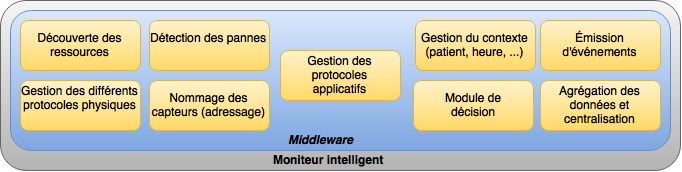
\includegraphics[width=1.5\textwidth]{Figure4.png}
	\caption{Middleware au niveau du Moniteur}
	\label{4}
\end{figure}

Ce requis impose de pouvoir comprendre différents protocoles, tant au niveau physique que applicatif, ainsi que différents formats. Il est en effet peu probable que tous les capteurs utilisent le même protocole pour leurs données sous un même format. Il est également nécessaire de permettre l'évolutivité au sein du système afin que de futurs capteurs plus performants, mais utilisant une nouvelle façon de communiquer, puissent être intégrés au système. Ceci sera géré par les modules de \textbf{\textit{gestion des différents protocoles physiques}} et \textbf{\textit{gestion des protocoles applicatifs}}.
\newline

De plus, afin d'optimiser le temps du personnel médical, il est souhaitable que le moniteur et donc le middleware facilite la découverte de capteurs ainsi que la récupération de leur contexte, ce qui sera rendu possible par le module de \textbf{\textit{découverte des ressources}}. Dans le TP1 nous avons évoqué la transmission de données depuis les capteurs. Pour que ces données aient une réelle signification, il faut que notre système soit conscient du type des données et des unités dans lesquelles ces données sont exprimées. Lorsqu’un capteur est rajouté au réseau des capteurs, c’est à dire qu’il s’enregistre auprès du moniteur intelligent, le capteur envoie ses propriétés, c’est à dire le type de données et l’unité associée. Le moniteur peut ainsi stocker dans sa table de correspondance le protocole physique, le canal de communication, le type de données et l’unité associée, ainsi que le nom que le moniteur intelligent attribue au capteur qui vient de s’enregistrer. Ce nom est transmis au capteur qui peut alors le retenir. Ce faisant, le moniteur est conscient, pour les données qu’il reçoit, de leur sémantique et des unités associées. Lors de l’agrégation des données et avant leur envoi à la Smart Gateway, le moniteur intelligent peut associer pour chaque type de données récupérées les unités associées dans un ou plusieurs paquets IPv4/IPv6 envoyés à la Smart Gateway. Ce processus est illustré par la Figure \ref{5}.
\newline
\begin{figure}[h!]
	\hspace*{-3cm}
	\centering
	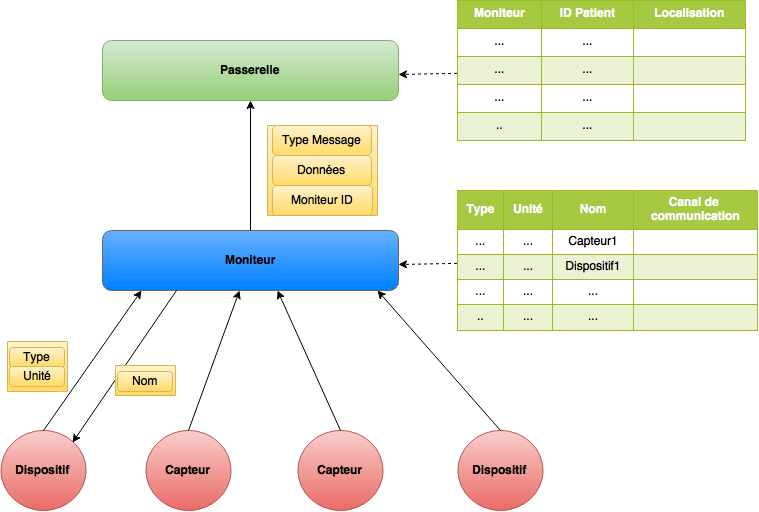
\includegraphics[width=1.5\textwidth]{Figure5.png}
	\caption{Découverte des Ressources et Gestion des Données}
	\label{5}
\end{figure}

Une fois les capteurs installés et découverts, le lien entre les données reçues, leurs unités et l'identité du patient devrait être fait automatiquement (ou presque), ce qu'assurera le module de \textbf{\textit{gestion du contexte}}. Cette étape intervient lorsque les données sont agrégées et préparées pour leur transmission par le module d'\textbf{\textit{agrégation des données}}.

Ces mêmes capteurs devraient être accessibles depuis l'extérieur. En effet, pour certaines données relevées rarement, il est possible qu'un médecin souhaite les rafraîchir plutôt que d'attendre la prochaine mise à jour. Il se peut également que le médecin, ou un outil automatique tel que le moniteur central, désire donner un ordre à un des objets intelligents. Pour cela, il faut que ces objets aient un nom, ou du moins soient adressables. En particulier, un nom du type \textit{idPatient@typeDeCapteur} serait particulièrement pratique à utiliser. Le module de \textbf{\textit{nommage des capteurs}} répondra à ce problème. De plus, il peut être nécessaire, dans le cas de décisions automatisées (par exemple la régulation d'un débit de perfusion, ...), que le middleware comprenne un \textbf{\textit{module de décision}} pour lequel des règles pourraient être définie afin qu'il actionne des objets connectés présents dans l'environnement du patient.
\newline

Enfin, il est impératif, dans la mesure du possible, de sécuriser les communications au sein du système. Cela passe par un
contrôle d'accès au niveau du moniteur avec un mécanisme d'authentification. Mais aussi par une \textbf{\textit{détection des pannes}}, dont un module s'occupe. En effet, il
est souhaitable que, de part l'importance des données fournies par ces capteurs, ils doivent être remplacés dès le premier indice
de dysfonctionnement. De manière générale, il est important de garantir une bonne disponibilité ainsi qu'une certaine fiabilité.
\newline

Ces considérations sur la détection de pannes entrainent également la nécessité de disposer d'un module d'\textbf{\textit{émission d'évènements}} afin que le middleware du moniteur intelligent puisse avertir immédiatement la Smart Gateway d'un dysfonctionnement d'un capteur, ou d'une valeur anormale par rapport au profil du patient (par exemple une crise cardiaque).
\newline

\begin{table}[h!]
	\hspace*{-4.5cm}
    \centering
    \begin{tabular}{|l|c|c|c|c|c|c|c|c|c|c|}
        \hline
        Modules & \begin{tabular}[c]{@{}l@{}} Découverte \\ ressources \end{tabular} & Scalabilité & \begin{tabular}[c]{@{}l@{}} Interopéra- \\ -bilité \end{tabular} & \begin{tabular}[c]{@{}l@{}} Adapta- \\ -bilité \end{tabular} & Fiabilité & \begin{tabular}[c]{@{}l@{}} Disponi- \\ -bilité \end{tabular} &  \begin{tabular}[c]{@{}l@{}} Temps \\
        réel \end{tabular} & \begin{tabular}[c]{@{}l@{}} Basé \\ sur les \\ services \end{tabular} &  \begin{tabular}[c]{@{}l@{}} Context \\ aware \end{tabular} & Autonome\\
        \hline
        \hline
        \begin{tabular}[c]{@{}l@{}}Découverte \\ des \\ ressources \end{tabular} & \checkmark & \checkmark & & \checkmark & & & & &&\\
        \hline
        \begin{tabular}[c]{@{}l@{}}Détection \\ panne \end{tabular} & & & & & \checkmark & \checkmark & \checkmark &  \checkmark && \\
        \hline
        Décision & & \checkmark & & \checkmark & \checkmark & \checkmark & & & & \checkmark \\
        \hline
        \begin{tabular}[c]{@{}l@{}}Gestion \\ du \\ contexte \end{tabular} & & & && & &&& & \checkmark \\
        \hline
        \begin{tabular}[c]{@{}l@{}}Émission \\ d'événements \end{tabular} & & & \checkmark & \checkmark & & \checkmark & & & \checkmark & \\
        \hline
        \begin{tabular}[c]{@{}l@{}}Gestion des \\ différents \\ protocoles \\ physiques \end{tabular} & & \checkmark & && & & & & & \\
        \hline
        \begin{tabular}[c]{@{}l@{}}Nommage \\ des capteurs \end{tabular} & & \checkmark & \checkmark & \checkmark && & & & & \\
        \hline
        \begin{tabular}[c]{@{}l@{}} Agrégation \\ de données et \\ centralisation  \end{tabular} & & \checkmark & \checkmark & \checkmark & & & & & & \\
        \hline
        \begin{tabular}[c]{@{}l@{}} Gestion des \\ différents \\ protocoles \\ applicatifs \end{tabular} & & \checkmark & \checkmark & \checkmark & & & & & &\\
        \hline
    \end{tabular}
    \caption{Utilisation des services du middleware par les différents modules}
\end{table}

\begin{table}[h!]
	\hspace*{-4cm}
    \centering
    \begin{tabular}{|l|c|c|c|c|}
        \hline
        Modules & Gestion ressources & Gestion données & Gestion événements & Gestion du code \\
        \hline
        \hline
        Découverte des ressources & \checkmark & & & \\
        \hline
        Détection panne & \checkmark & & & \\
        \hline
        Décision & & & &\\
        \hline
        Gestion du contexte & & \checkmark & \checkmark & \\
        \hline
        Émission d'événements & & \checkmark & \checkmark & \\
        \hline
        Gestion des différents protocoles physiques & & & & \checkmark \\
        \hline
        Nommage des capteurs & \checkmark & & & \\
        \hline
        Agrégation de données et centralisation & & \checkmark & & \\
        \hline
        Gestion des différents protocoles applicatifs & & & & \checkmark \\
        \hline
    \end{tabular}
    \caption{Utilisation des services de gestion du middleware par les différents modules}
\end{table}

Les tableaux 1 et 2 présentent les modules sur la première colonne avec les exigences du middleware sur la première ligne.
\newline

Par ailleurs, il serait aussi nécessaire de présenter une API simple d'utilisation au niveau du middleware afin de faciliter la programmation de nouvelles fonctionnalités et l'utilisation des services offerts par des applications extérieures.
